\chapter{光晶格系统中的动力学对称性}

这一章,我们来讨论光晶格系统中的动力学演化和动力学对称性的问题。作为具体的切入点,我们讨论关于一大类 Hubbard 模型的动力学演化和动力学对称性问题。作为凝聚态物理中许多问题的核心,同时也是超冷原子物理量子模拟的热点,Hubbard 模型本身受到了来自理论层面和实验层面的丰富的研究。 
这一章所讨论的动力学对称性问题为研究 Hubbard 模型的动力学演化提供了新的思路、方法、和视角。

我们将介绍 有 Hubbard 相互作用的体系中一类受保护的动力学对称性(\ref{sec:dynsymm}),和 一类 Fermi-Hubbard 模型中 的 电荷密度波和自旋密度波 的动力学演化,以及相应的电荷输运和自旋输运性质的对称性(\ref{sec:diffusion}),以及证明相关定理。这两个定理给超冷原子物理中的一些实验现象\cite{hubbard-expan-2010,hubbard-expan-2012,mbl1d,twobody-2017,charge-diffusion,spin-diffusion}给出了全新的理解,和可供借鉴的角度。



\section{有 Hubbard 相互作用体系中 受保护的 动力学对称性}\label{sec:dynsymm}

考虑一类有 Hubbard 相互作用的体系。描述这类体系的哈密顿量为如下形式
\begin{align}
\hat{H} = \hat{H}_0 + \hat{H}_I
\end{align}
其中 $H_0$ 为单粒子哈密顿量,$H_I$ 为有格点上的 Hubbard 相互作用的相互作用项。对于自旋1/2的费米子来说,
\begin{align}
\hat{H}_I=U\sum_j\hat{n}_{j\uparrow}\hat{n}_{j\downarrow}
\end{align}
而对于玻色子来说,
\begin{align}
\hat{H}_I=U\sum_{j}\hat{n}_j(\hat{n}_j-1)/2
\end{align}
这其中 $U$ 代表了格点上相互作用的强度。
单粒子哈密顿量部分 $\hat{H}_0$ 可能会存在对称性。我们发现,当 $\hat{H}_0$ 具有某些满足一定条件的对称性时,这类 Hubbard 系统衍生出一种动力学对称性,即在排斥相互作用($+U$)时的动力学演化和在吸引相互作用($-U$)时的动力学演化具有某种对称性。这种衍生的动力学对称性受单粒子哈密顿量 $\hat{H}_0$ 的对称性的保护(支持),我们也称之为对称性保护的动力学对称性\cite{dynsymm}。下面这个定理表达了这种动力学对称性。
\begin{theorem}\label{thm:dynsymm}
对于如 $\hat{H} = \hat{H}_0 + \hat{H}_I$ 形式的哈密顿量,我们考虑某个初态 $|\psi_i\rangle$ 在其主导下的幺正演化 $|\psi(t)\rangle = e^{\ii\hat{H}t}|\psi_i\rangle$,并且考虑某个可观测量 $\hat{O}$ 在该态下的期望值随时间的演化 $\langle\hat{O}(t)\rangle$。若存在一个幺正算符 $\hat{W}$,使得对$\hat{S}=\hat{R}\hat{W}$,$\hat{R}$ 为(反幺正的)时间反演算符,有
\begin{align}
\{\hat{S}, \hat{H}_0\} &= 0\\
[\hat{S}, \hat{H}_I] &= 0
\end{align}
且 $\hat{O}$ 是 $\hat{S}$-对称的,即
\begin{align}
\hat{S}\hat{O}\hat{S}^{-1} = \pm \hat{O}
\end{align}
和 $|\psi_i\rangle$ 是 $\hat{S}$-不变的,即
\begin{align}
\hat{S}|\psi_i\rangle = e^{\ii\chi}|\psi_i\rangle
\end{align}
那么, $\langle\hat{O}(t)\rangle$ 具有 $U\leftrightarrow-U$ 的对称性:
\begin{align}
\langle\hat{O}(t)\rangle_{+U} = \pm\langle\hat{O}(t)\rangle_{-U}
\end{align}
式中的正负号取决于 $\hat{O}$ 关于 $\hat{S}$ 是奇对称还是偶对称(即$\hat{S}\hat{O}\hat{S}^{-1} = \pm \hat{O}$ 的正负号)。
\end{theorem}

\begin{proof}
直接验证,
\begin{align}
\langle \hat{O}(t)\rangle_{+U}&=\langle\psi_i|e^{\ii \hat{H}t}\hat{O}e^{-\ii \hat{H}t}|\psi_i\rangle\\
&=\langle\psi_i|e^{\ii (\hat{H}_0+\hat{H}_I[U])t}\hat{O}e^{-\ii (\hat{H}_0+\hat{H}_I[U])t}|\psi_i\rangle\\
&=\langle\psi_i|\hat{S}^{-1}\hat{S}e^{\ii (\hat{H}_0+\hat{H}_I[U])t}\hat{S}^{-1}\hat{S}\hat{O}\hat{S}^{-1}\hat{S}e^{-\ii (\hat{H}_0+\hat{H}_I[U])t}\hat{S}^{-1}\hat{S}|\psi_i\rangle\\
&=\langle\psi_i|e^{-\ii\chi}e^{-\ii (-\hat{H}_0+\hat{H}_I[U])t}(\pm \hat{O})e^{\ii (-\hat{H}_0+\hat{H}_I[U])t}e^{\ii\chi}|\psi_i\rangle\\
&=\pm\langle\psi_i|e^{\ii (\hat{H}_0-\hat{H}_I[U])t}\hat{O}e^{-\ii (\hat{H}_0-\hat{H}_I[U])t}|\psi_i\rangle\\
&=\pm\langle\psi_i|e^{\ii (\hat{H}_0+\hat{H}_I[-U])t}\hat{O}e^{-\ii (\hat{H}_0+\hat{H}_I[-U])t}|\psi_i\rangle\\
&=\pm\langle \hat{O}(t)\rangle_{-U}
\end{align}
证毕。
\end{proof}

以上定理对满足对称性条件的混态系综也是成立的。

\begin{corollary}
对于一混合初态,密度矩阵写作 
\begin{align}
\rho_i=\sum_jp_j|\psi_j\rangle\langle\psi_j|
\end{align}
若其中混合的每一个纯态 $|\psi_j\rangle$ 均为 $\hat{S}$-不变的,则该混态满足以上定理 \ref{thm:dynsymm} 的条件,即,对同样满足定理 \ref{thm:dynsymm} 条件的 $\hat{H}$ 和 $\hat{O}$ 上述定理结论成立。
\end{corollary}

\begin{proof}
直接验证,
\begin{align}
\langle \hat{O}(t)\rangle_{\rho_i,+U}&=Tr(\rho_i\hat{O}_{+U}(t))\\
&=\sum_{j}p_j\langle \hat{O}(t)\rangle_{j,+U}\\
&=\sum_jp_j(\pm)\langle \hat{O}(t)\rangle_{j,-U}\\
&=Tr(\pm\rho_i\hat{O}_{-U}(t))\\
&=\pm \langle \hat{O}(t)\rangle_{\rho_i,-U}
\end{align}
证毕。
\end{proof}

对于这个定理,我们给出三类具有代表性的例子进行展示。这三类例子分别对应定理中关于 哈密顿量$\hat{H}$,初态 $|\psi_i\rangle$,和可观测算符 $\hat{O}$ 需满足的三个条件,也分别对应着近年来在冷原子物理中的几个实验\cite{hubbard-expan-2010,hubbard-expan-2012,mbl1d,twobody-2017}。


\subsection{Fermi Hubbard 模型:不同的晶格几何}
首先考虑正方晶格上的 Fermi Hubbard 模型\cite{hubbard-expan-2010,hubbard-expan-2012}。其哈密顿量写作
\footnote{以下在不致混淆的情况下,对算符上的尖帽均隐含不写。}
\begin{align}
    H=-\sum_{\langle i,j\rangle,\sigma}t_{ij}c_{i\sigma}^{\dagger}c_{j\sigma}+h.c.+\sum_iUn_{i\uparrow}n_{i\downarrow}
\end{align}
晶格结构如图 \ref{fig:dynm:fhsquare} 所示。
\begin{figure}[!htb]
\centering
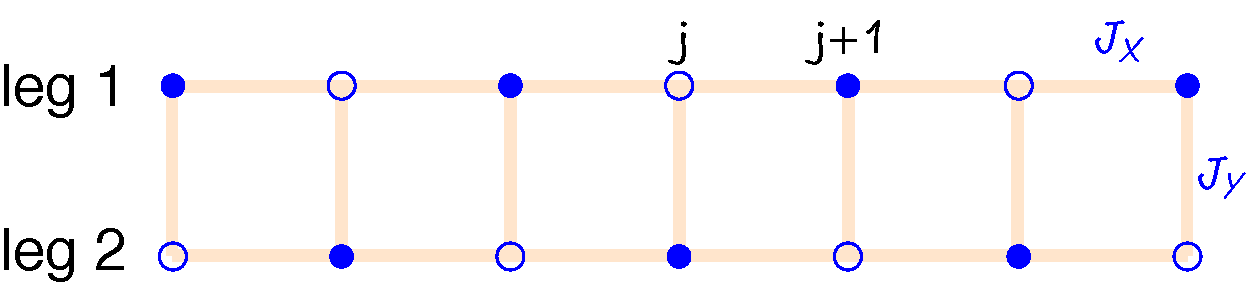
\includegraphics[width=1.0\columnwidth]{chap3_dynm/fhsquare}
\caption{正方晶格上的 Fermi Hubbard 模型示意图。可以看出,正方晶格是二分(bipartite)晶格,意味着晶格可以分为两套$A/B$子格,且每套子晶格中的每个格点只和另一套晶格中的格点相连。}
\label{fig:dynm:fhsquare}
\end{figure}
对该哈密顿量,有如下的幺正变换 $\hat{W}$ 和 时间反演变换 $\hat{R}$,
\begin{align}
& W: \, c_{l\sigma}\rightarrow (-1)^lc_{l\sigma} \\
& K: \,\ii\rightarrow-\ii \\
& R = \ii\sigma_yK 
\end{align}
使得\footnote{这与正方晶格是二分(bipartite)晶格有密切关系。更具体来说,对二分晶格可以定义手征算符 $\Gamma=P_A-P_B$,满足 $\{\Gamma, H_0\}=0$。这使得二分晶格的单粒子谱是正负对称的。一个著名的这样的例子是 SSH 模型。}
\begin{align}
WH_0W^{-1} &= -H_0 \\ 
WH_IW^{-1} &= H_I
\end{align}
继而对 $S=RW$ 有
\begin{align}
SH_0S^{-1} &= -H_0 \\ 
SH_IS^{-1} &= H_I
\end{align}
现在我们来考虑下面这样的初态,
\begin{align}
    |\psi_i\rangle=\sum_j (-1)^jc_{j\uparrow}^{\dagger}c_{j\downarrow}^{\dagger}|0\rangle
\end{align}
容易验证初态在 $S$ 作用下是不变的。同时,我们考虑局域密度的演化,$\langle n_l(t)\rangle$,作为我们的可观测量,那么依据定理 \ref{thm:dynsymm},其含时演化对于排斥相互作用和吸引相互作用具有对称性。且,因 $n_l$ 在 $S$ 下是偶对称的,
\begin{align}
Sn_lS = n_l
\end{align}
应有
\begin{align}
\langle n_l(t)\rangle_{+U} = \langle n_l(t)\rangle_{-U}
\end{align}
我们对 $2\times15$ 个格点的周期性边界条件的体系进行了数值验证。进行严格对角化(Exact Diagonalization,ED)计算,得到几个局域密度观测量在一段时间内的演化,如图 \ref{fig:dynm:fhsed} 所示。
\begin{figure}[!htb]
\begin{subfigure}{.5\textwidth}
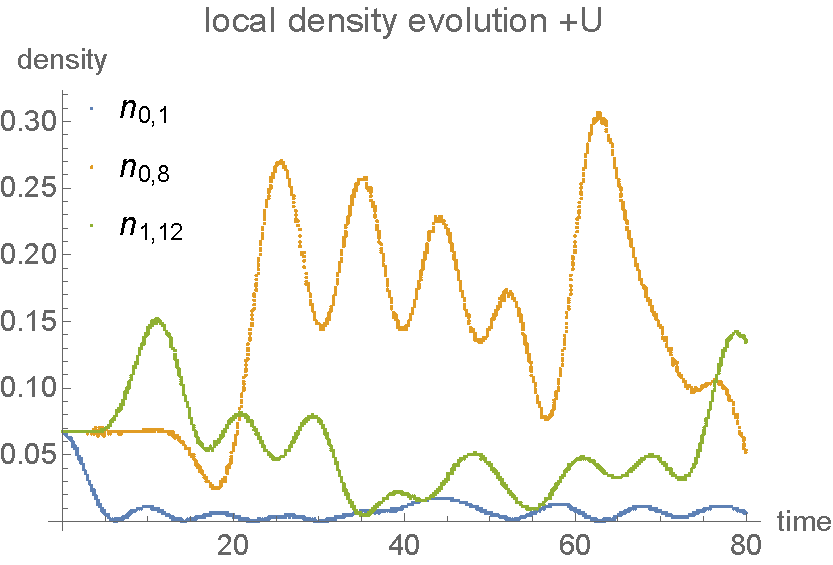
\includegraphics[width=1.\columnwidth]{chap3_dynm/fig_fh1.pdf}
\end{subfigure}
\begin{subfigure}{.5\textwidth}
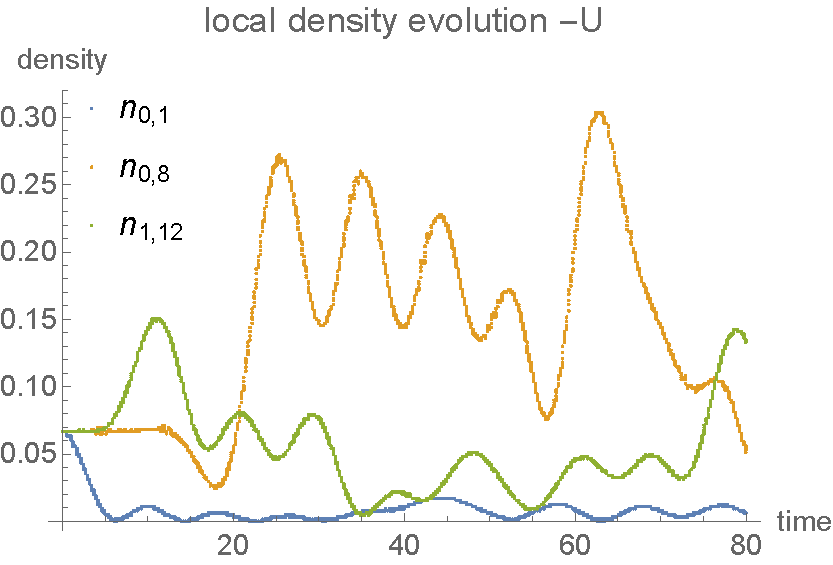
\includegraphics[width=1.\columnwidth]{chap3_dynm/fig_fh2.pdf}
\end{subfigure}\\
\begin{subfigure}{.5\textwidth}
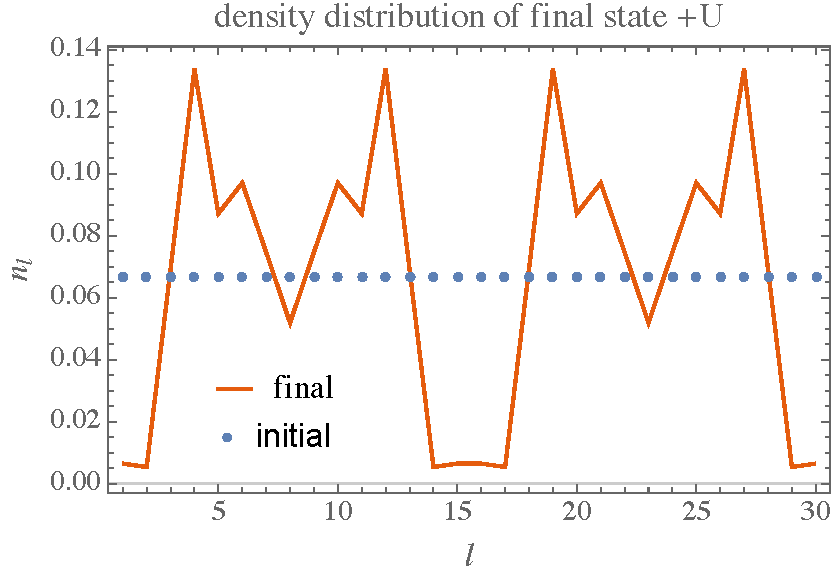
\includegraphics[width=1.\columnwidth]{chap3_dynm/fig_fh3.pdf}
\end{subfigure}
\begin{subfigure}{.5\textwidth}
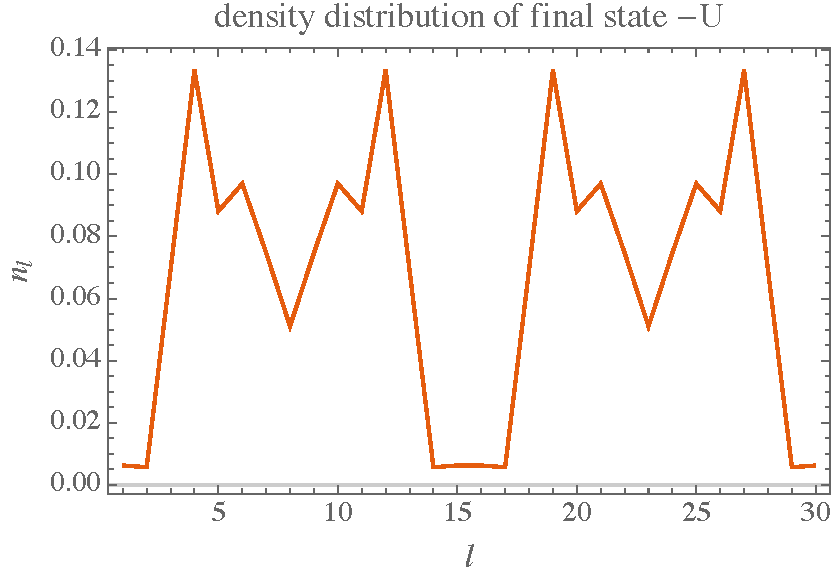
\includegraphics[width=1.\columnwidth]{chap3_dynm/fig_fh4.pdf}
\end{subfigure}
\caption{正方晶格 Fermi Hubbard 模型局域密度观测量的演化。左栏为 $+U$下的演化,右栏为 $-U$下的演化。晶格大小为 $2\times15$ 个格点,周期性边界条件,模型参数为 $J_Y/J_X=1$, $|U|/J_X=10$,初态为 $|\psi_i\rangle=\sum_j (-1)^jc_{j\uparrow}^{\dagger}c_{j\downarrow}^{\dagger}|0\rangle$。横轴时间单位上 $\hbar$ 取作1.}
\label{fig:dynm:fhsed}
\end{figure}

由图 \ref{fig:dynm:fhsed} 所见,数值验证的结果显示,在正方晶格 Fermi Hubbard 模型中,局域密度观测量在该态演化下的期望值确实具有 $+U/-U$ 的对称性,且为偶对称。



下面来考虑三角晶格上的 Fermi Hubbard 模型。哈密顿量写作
\begin{align}
    H=-\sum_{i,j,\sigma}J_Xc_{i,j+1,\sigma}^{\dagger}c_{i,j,\sigma}+J_Yc_{1,j,\sigma}^{\dagger}c_{0,j,\sigma}+J_Yc_{1,j+1,\sigma}^{\dagger}c_{0,j,\sigma}+H.c.+\sum_iUn_{i\uparrow}n_{i\downarrow}
\end{align} 
晶格结构如图 \ref{fig:dynm:fhtriangle} 所示。
\begin{figure}[!htb]
\centering
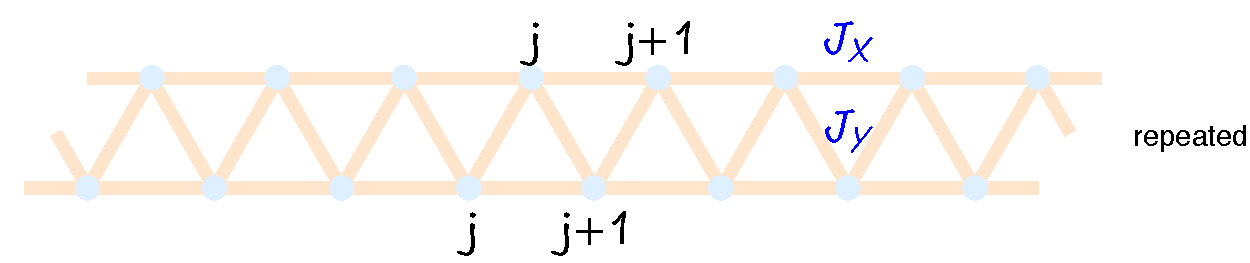
\includegraphics[width=1.0\columnwidth]{chap3_dynm/fhtriangle}
\caption{三角晶格上的 Fermi Hubbard 模型示意图。三角晶格不是二分晶格,无法分成$A/B$ 两套子格使其满足每套子晶格中的每个格点只和另一套晶格中的格点相连。}
\label{fig:dynm:fhtriangle}
\end{figure}

对于三角晶格,上述 $W$ 和 $S$ 将不再满足定理条件,哈密顿量在 $S$ 下不具有上面描述的对称性。因此可以预见,定理结论不再成立,即,选择同样初态和同样的可观测算符,如局域密度算符,其随时间演化的期望值不具有 $+U/-U$ 对称性。

作为验证,我们同样进行了严格对角化(ED)计算,同样对于一个 $2\times15$ 大小周期性边界条件的晶格。如图 \ref{fig:dynm:fhted} 所示,局域密度可观测量在该态下的期望值确实不再具有 $+U/-U$ 对称性。

\begin{figure}[!htb]
\begin{subfigure}{.5\textwidth}
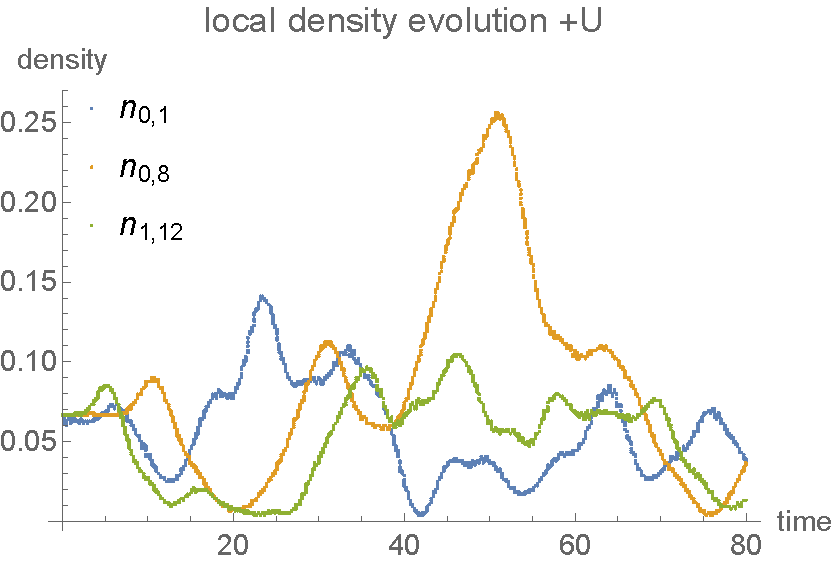
\includegraphics[width=1.\columnwidth]{chap3_dynm/fig_fhtri1.pdf}
\end{subfigure}
\begin{subfigure}{.5\textwidth}
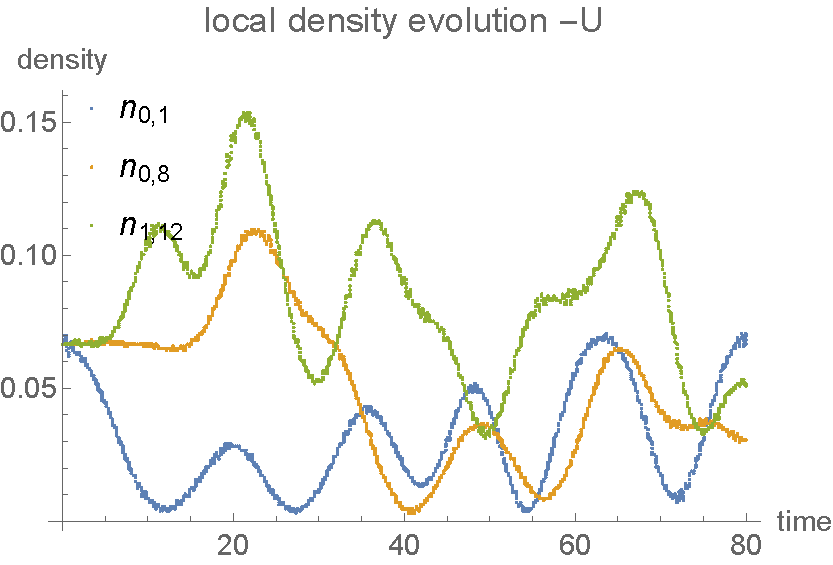
\includegraphics[width=1.\columnwidth]{chap3_dynm/fig_fhtri2.pdf}
\end{subfigure}\\
\begin{subfigure}{.5\textwidth}
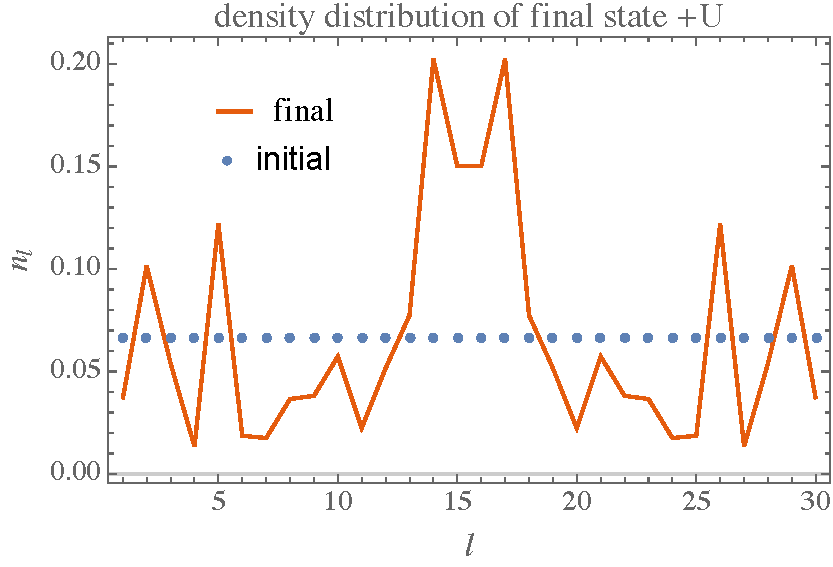
\includegraphics[width=1.\columnwidth]{chap3_dynm/fig_fhtri3.pdf}
\end{subfigure}
\begin{subfigure}{.5\textwidth}
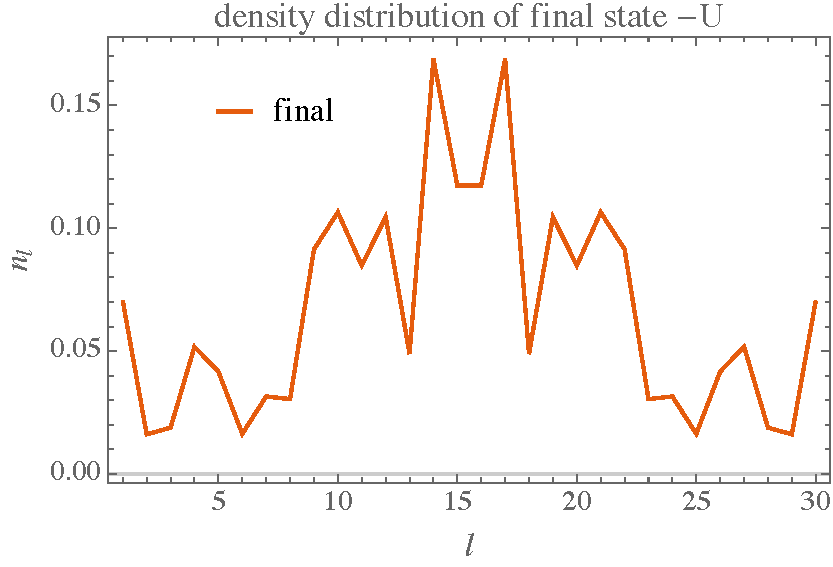
\includegraphics[width=1.\columnwidth]{chap3_dynm/fig_fhtri4.pdf}
\end{subfigure}
\caption{三角晶格 Fermi Hubbard 模型局域密度观测量的演化。左栏为 $+U$下的演化,右栏为 $-U$下的演化。晶格大小为 $2\times15$ 个格点,周期性边界条件,模型参数为 $J_Y/J_X=1$, $|U|/J_X=10$,初态为 $|\psi_i\rangle=\sum_j (-1)^jc_{j\uparrow}^{\dagger}c_{j\downarrow}^{\dagger}|0\rangle$。横轴时间单位上 $\hbar$ 取作1.}
\label{fig:dynm:fhted}
\end{figure}



\subsection{玻色子带磁通的 Hubbard 晶格:不同的初态}
下面来考虑在正方晶格上玻色子的带磁通的的 Hubbard 模型\cite{twobody-2017}。哈密顿量写作
\begin{align}
H=&-\sum_jJ_X(e^{-\ii\phi/2}a^{\dagger}_{j+1}a_j+e^{\ii\phi/2}b^{\dagger}_{j+1}b_j)+J_Ya_j^{\dagger}b_j+h.c. 
% \\&\qquad\qquad\qquad\qquad
+\dfrac{U}{2}\sum_jn_j^{(a)}(n_j^{(a)}-1)+n_j^{(b)}(n_j^{(b)}-1)
\end{align}
晶格结构如图 \ref{fig:dynm:fluxladder} (a) 所示。
\begin{figure}[!htb]
\centering
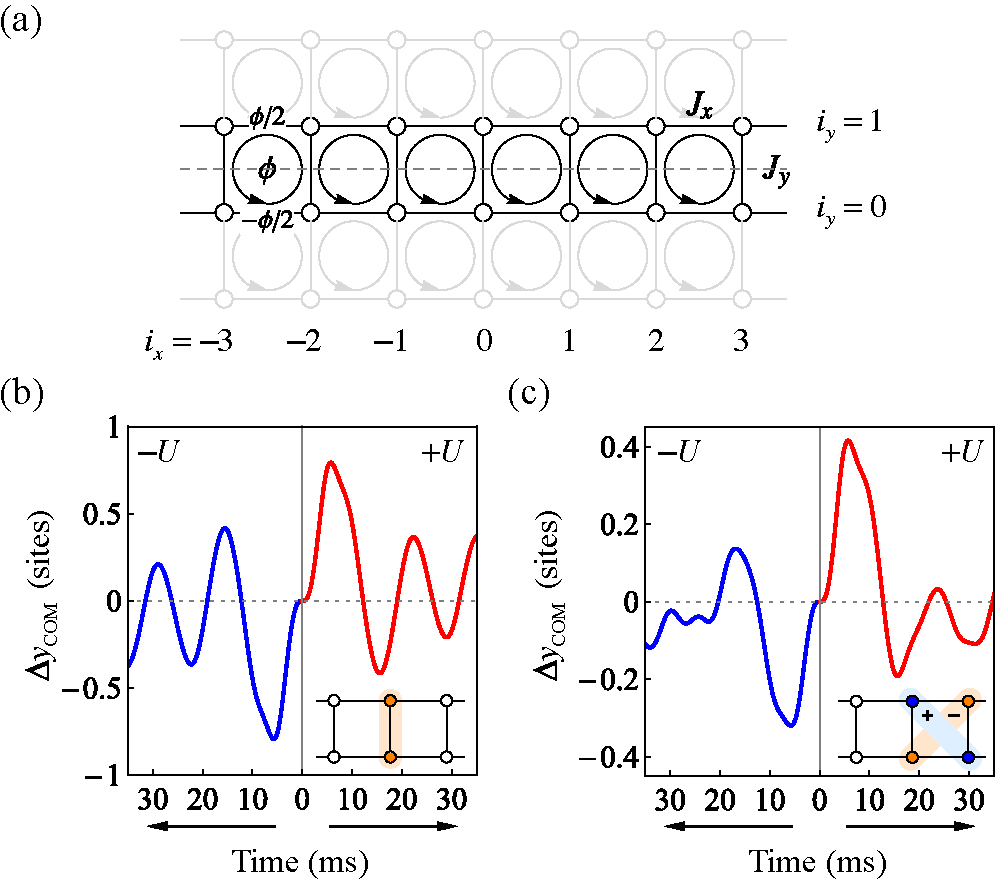
\includegraphics[width=1.0\columnwidth]{dynsymm/example2}
\caption{正方晶格上玻色子的带磁通的的 Hubbard 模型。(a) 晶格结构示意图;(b)初态 \ref{eq:state1} 演化下 $\Delta y_{\text{c.m.}}(t)$ 期望值;(c)初态 \ref{eq:state2} 演化下 $\Delta y_{\text{c.m.}}(t)$ 的期望值。 模型参数见 \inlinecite{dynsymm}(取自\inlinecite{dynsymm})}
\label{fig:dynm:fluxladder}
\end{figure}
考虑如下的幺正变换
\begin{align}
&\hat{W}^{-1}\hat{c}_{i_x,i_y,\sigma}\hat{W}=(-1)^{i_x+i_y}\hat{c}_{i_x,1-i_y,\sigma},  \label{W2} 
\end{align}
容易验证,该幺正变换满足定理 \ref{thm:dynsymm} 所述条件\cite{dynsymm}。
先考虑如下两种初态。第一种
\begin{align}\label{eq:state1}
|\Psi_0\rangle&=\frac{1}{2}(\hat{c}^\dag_{0,0}+\hat{c}^\dag_{0,1})(\hat{c}^\dag_{0,0}-\hat{c}^\dag_{0,1})|0\rangle\nonumber\\
&=\hat{c}^\dag_{0,0}\hat{c}^\dag_{0,1}|0\rangle.
\end{align}
容易验证,该算符具有 $S$-不变性。现在考虑以该态作为初态的幺正演化,演化一段时间后其左右两半的质心(Center-of-Mass)位置的期望值,定义如下的观测量
\begin{align}
\Delta y_{\text{c.m.}}(t)=\frac{\langle \hat{O}^R_{-}(t)\rangle}{\langle \hat{O}^R_{+}(t)\rangle}-\frac{\langle \hat{O}^L_{-}(t)\rangle}{\langle \hat{O}^L_{+}(t)\rangle}
\end{align}
其中
\begin{align}
&\hat{O}^R_{\pm}=\sum\limits_{i_x>0}(\hat{n}_{i_x,i_y=1}\pm \hat{n}_{i_x,i_y=0}), \\
&\hat{O}^L_{\pm}=\sum\limits_{i_x<0}(\hat{n}_{i_x,i_y=1}\pm \hat{n}_{i_x,i_y=0}). 
\end{align}
可以直接验证,
\begin{align}
\hat{S}^{-1}\hat{O}^{R/L}_{\pm}\hat{S}=\pm \hat{O}^{R/L}_{\pm},
\end{align}
因此,
\begin{align}
\Delta y_{\text{c.m.}}(t)|_{+U}=-\Delta y_{\text{c.m.}}(t)|_{-U}
\end{align}
对此,我们做了数值检验。经过严格对角化计算,该态下的 $\Delta y_{\text{c.m.}}(t)$ 期望值确实具有 $+U/-U$ 对称性,且为奇对称,如图 \ref{fig:dynm:fluxladder}(b) 所示。

现在考虑另一种初态,
\begin{align}\label{eq:state2}
|\Psi_0\rangle&=\frac{1}{2}(\hat{c}^\dag_{0,1}+\hat{c}^\dag_{1,0})(\hat{c}^\dag_{1,1}-\hat{c}^\dag_{0,0})|0\rangle,
\end{align}
可以直接验证,该态并不具备定理 \ref{thm:dynsymm} 所述 $S$-不变性,因此定理结论不成立,$\Delta y_{\text{c.m.}}(t)$ 在其演化下的期望值不具有 $+U/-U$ 对称性。数值模拟结果见图 \ref{fig:dynm:fluxladder} (c)。




\subsection{Aubry-Andre 模型:不同的可观测量的对称性}
下面来考虑 Aubry-Andre 模型。模型的哈密顿量写作
\begin{align}
\hat{H}_0=\sum\limits_{i,\sigma}-J(\hat{c}^\dag_{i,\sigma}\hat{c}_{i+1,\sigma}+\text{h.c.})+\Delta\cos(2\pi\beta i+\theta)\hat{n}_{i,\sigma} + U\sum_j\hat{n}_{j\uparrow}\hat{n}_{j\downarrow}
\end{align}
晶格结构如图 \ref{fig:dynm:aa} (a) 所示。这是一个利用不公度的晶格实现准无序体系的模型\cite{mbl1d}。
\begin{figure}[!htb]
\centering
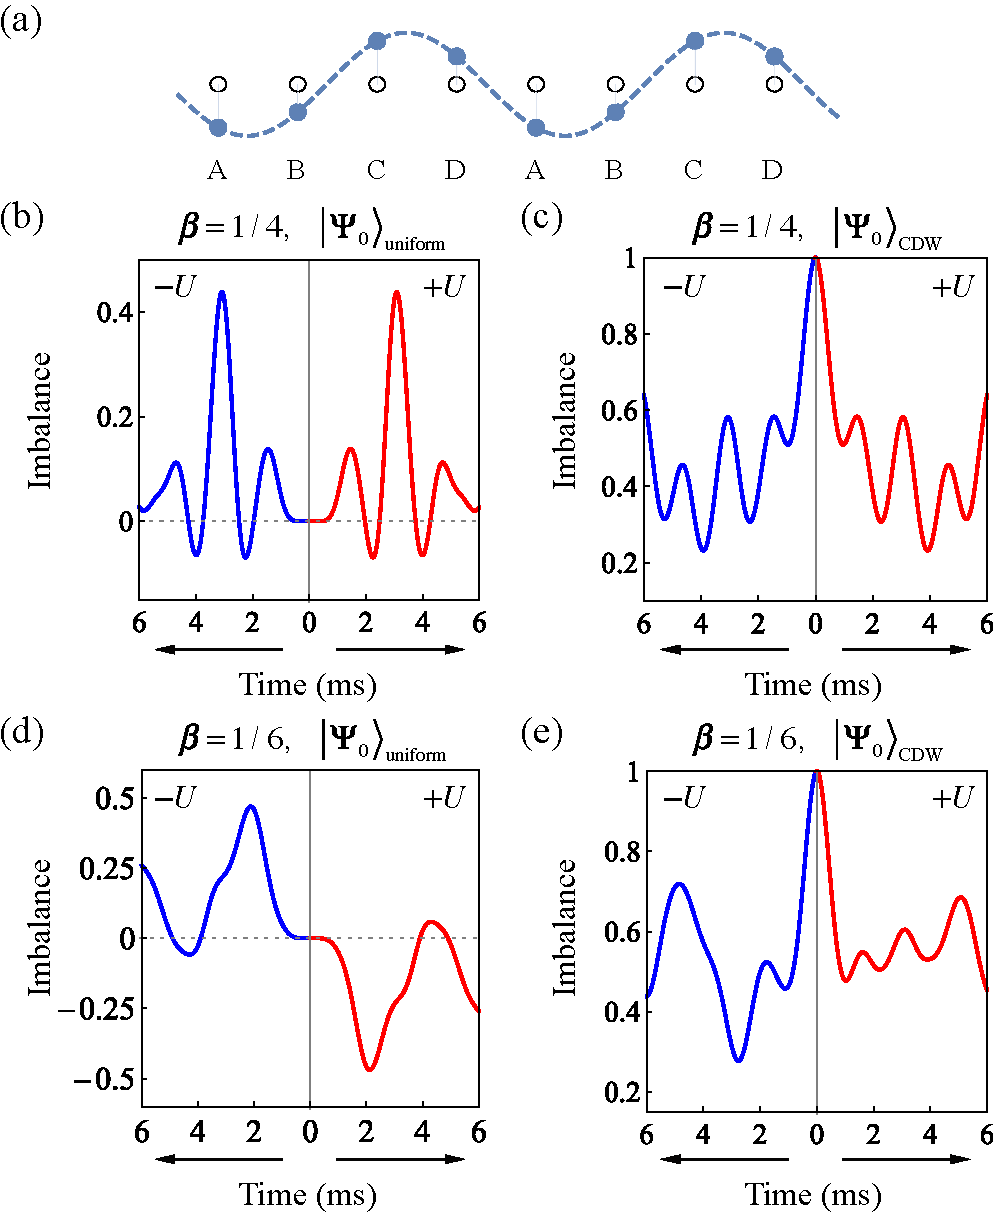
\includegraphics[width=1.0\columnwidth]{dynsymm/example3}
\caption{Aubry-Andre Hubbard 模型。(a) 晶格结构示意图;(b)(c) $\beta=1/4$ 时,两种初态演化下非平衡观测量的期望值;(d)(e) $\beta=1/6$ 时,两种初态演化下非平衡可观测量的期望值。利用严格对角化进行数值模拟。模型参数见 \inlinecite{dynsymm}(取自\inlinecite{dynsymm})}
\label{fig:dynm:aa}
\end{figure}

现在考虑一种非平衡观测量\cite{mbl1d},定义如下
\begin{equation}
\hat{\mathcal{I}}=\frac{\sum_{i\subset \text{even}}\hat{n}_{i\sigma}-\sum_{i\subset \text{odd}}\hat{n}_{i\sigma}}{\sum_{i\subset \text{even}}\hat{n}_{i\sigma}+\sum_{i\subset \text{odd}}\hat{n}_{i\sigma}}.
\end{equation}
和两种初态,
\begin{align}
&|\Psi_0\rangle_{\text{uniform}}=\frac{1}{\sqrt{N}}\sum\limits_{i=1}^{N}\hat{c}^\dag_{i\uparrow}\hat{c}^\dag_{i\downarrow}|0\rangle;\\
&|\Psi_0\rangle_{\text{CDW}}=\frac{1}{\sqrt{N/2}}\sum\limits_{i=1,i\subset \text{odd}}^{N}\hat{c}^\dag_{i\uparrow}\hat{c}^\dag_{i\downarrow}|0\rangle.
\end{align}
考虑该可观测量在这两种态的幺正演化下的期望值。为了发现其动力学演化的精确关系,我们现在利用定理 \ref{thm:dynsymm}。现在需要找到合适的 $\hat{S}$ 也就是 $\hat{W}$。

这里的晶格不公度参数 $\beta$ 总可以写为有理数,或用有理数近似逼近。即 
\begin{align}
\beta=p/q
\end{align}
对 $p,q$ 不同的情况,我们寻找不同的 $\hat{W}$。
\begin{enumerate}
\item $p$ 是奇数,$q$ 是偶数,且 $q/2$ 是偶数。
存在
\begin{align}
\hat{W}^{-1}\hat{c}_{i,\sigma}\hat{W}=(-1)^{i}\hat{c}_{i+q/2,\sigma}.  \label{W3} 
\end{align}
模型在其变换下具有不变性。
使得 $\hat{\mathcal{I}}$ 在 $\hat{S}$ 下是偶对称,且 $|\Psi_0\rangle_{\text{uniform}}$ 和 $|\Psi_0\rangle_{\text{CDW}}$ 态均为 $\hat{S}$-不变的。因此,这种情况下,$\hat{\mathcal{I}}$ 在两种初态幺正演化下的期望值均有 $+U/-U$ 对称性,且为偶对称。见图 \ref{fig:dynm:aa}(b)(c)。

\item $p$ 是奇数,$q$ 是偶数,且 $q/2$ 是奇数。
这时,上式的 $\hat{W}$ 还是满足模型的对称性的。但此时,$\hat{\mathcal{I}}$ 在 $\hat{S}$ 下是奇对称,且只有 $|\Psi_0\rangle_{\text{uniform}}$ 在其下不变,$|\Psi_0\rangle_{\text{CDW}}$ 在其变换下不再具有不变性。因此,这种情况下,$\hat{\mathcal{I}}$ 在 $|\Psi_0\rangle_{\text{uniform}}$ 幺正演化下的期望值具有 $+U/-U$ 对称性,且为奇对称,而在 $|\Psi_0\rangle_{\text{CDW}}$ 幺正演化下的期望值不再具有 $+U/-U$ 对称性。见图 \ref{fig:dynm:aa}(d)(e)。

\item $q$ 是奇数。这种情况下无法找到满足定理 \ref{thm:dynsymm} 所述的 $\hat{S}$。非平衡可观测量的演化不具有 $+U/-U$ 对称性。
\end{enumerate}



\section{Fermi-Hubbard 模型中电荷输运与自旋输运的对称性}\label{sec:diffusion}

Fermi Hubbard 模型中的电荷输运与自旋输运问题是许多凝聚态物理所关注的问题的核心。特别是,最近在冷原子物理中也有若干实验研究在光晶格模拟中的电荷输运问题\cite{charge-diffusion}和自旋输运问题\cite{spin-diffusion},并对电荷输运扩散系数和自旋输运扩散系数\cite{spin-diffusion}进行了研究。

受上述实验的启发,我们发现了在一类二分晶格 Fermi Hubbard 模型中电荷和自旋在动力学性质方面的对称性\cite{diffusion}。下面我们将讨论这种对称性,并给出一定的精确关系。

我们考虑二分晶格上的 Fermi Hubbard 模型,其哈密顿量写作
\begin{align}
    \hat{H} = \sum_{\langle i,j\rangle,\sigma} -t\hat{c}_{i\sigma}^{\dagger}\hat{c}_{j\sigma} + \sum_{i} U \hat{n}_{i\uparrow}\hat{n}_{i\downarrow} 
\end{align}
这里 $\langle i,j\rangle$ 标示最近邻格点,其中 $i\in A$ 而 $j\in B$。

如果考虑多体系统,则可以通过调节化学势来改变体系的总粒子数。这是可将哈密顿量写作
\begin{align}
    \hat{H} = \sum_{\langle i,j\rangle,\sigma} -t\hat{c}_{i\sigma}^{\dagger}\hat{c}_{j\sigma} + \sum_{i} U \hat{n}_{i\uparrow}\hat{n}_{i\downarrow} - \sum_i\mu_i\hat{n}_i
\end{align}
这里 $\mu_i$ 是局域的化学势,或者
\begin{align}
    \hat{H} = \sum_{\langle i,j\rangle,\sigma} -t\hat{c}_{i\sigma}^{\dagger}\hat{c}_{j\sigma} + \sum_{i} U \hat{n}_{i\uparrow}\hat{n}_{i\downarrow} -\mu\hat{N}
\end{align}
这里 $\mu$ 是总化学势。对于一个半填充的体系,$\mu=N/2$,或者说,
\begin{align}
    \hat{H} = \sum_{\langle i,j\rangle,\sigma} -t\hat{c}_{i\sigma}^{\dagger}\hat{c}_{j\sigma} + \sum_{i} U \left(\hat{n}_{i\uparrow}-\dfrac{1}{2}\right)\left(\hat{n}_{i\downarrow}-\frac{1}{2}\right) 
\end{align}

现在定义一组粒子空穴变换,
\begin{definition}
粒子空穴变换 $\mathcal{P}$ 为:
\begin{align}
    \mathcal{P} : \  \  
    & \hat{c}_{i\uparrow} \rightarrow (-1)^{i} \hat{c}_{i\uparrow}^{\dagger},  \nonumber\\
    & \hat{c}_{i\downarrow} \rightarrow \hat{c}_{i\downarrow}. 
\end{align}
\end{definition}
或者更具体可以写作,
\begin{align}
    \mathcal{P} |n_{i\uparrow} = 0\rangle = |n_{i\uparrow} = 1\rangle, \  \  
    \mathcal{P} |n_{i\uparrow} = 1\rangle = |n_{i\uparrow} = 0\rangle. 
\end{align}

\begin{lemma}\label{lemma1}
对于半填充的二分 Fermi Hubbard 模型,上述粒子空穴变换将 $+U$ 的模型映射为 $-U$ 的模型,以及反之。
\begin{align}
\mathcal{P}: H(+U) \leftrightarrow H(-U)
\end{align}
\end{lemma}

\begin{proof}
由 $\mathcal{P}$ 的定义易得,
\begin{align}
\mathcal{P}\left(\sum_{\langle i,j\rangle,\sigma} -t\hat{c}_{i\sigma}^{\dagger}\hat{c}_{j\sigma}\right) \mathcal{P}^{-1} = \sum_{\langle i,j\rangle,\sigma} -t\hat{c}_{i\sigma}^{\dagger}\hat{c}_{j\sigma} 
\end{align}
而对所有格点 $i$ 都有
\begin{align}
\mathcal{P}\left(\hat{n}_{i\uparrow}-\dfrac{1}{2}\right)\left(\hat{n}_{i\downarrow}-\frac{1}{2}\right) \mathcal{P}^{-1} &= \left(\dfrac{1}{2}-\hat{n}_{i\uparrow}\right)\left(\hat{n}_{i\downarrow}-\frac{1}{2}\right) \\
&= - \left(\hat{n}_{i\uparrow}-\dfrac{1}{2}\right)\left(\hat{n}_{i\downarrow}-\frac{1}{2}\right)
\end{align}
因此有
\begin{align}
\mathcal{P} \left(\sum_{i} U \left(\hat{n}_{i\uparrow}-\dfrac{1}{2}\right)\left(\hat{n}_{i\downarrow}-\frac{1}{2}\right) \right) \mathcal{P}^{-1} = - \sum_{i} U \left(\hat{n}_{i\uparrow}-\dfrac{1}{2}\right)\left(\hat{n}_{i\downarrow}-\frac{1}{2}\right) 
\end{align}
即,
\begin{align}
\mathcal{P}H(+U)\mathcal{P}^{-1} = H(-U)
\end{align}
证毕。
\end{proof}

现引入局域电荷密度算符和局域自旋密度算符的定义。
\begin{definition}
局域电荷密度算符 $\hat{n}_{i}$ 定义为 $\hat{n}_{i} = \hat{n}_{i\uparrow} + \hat{n}_{i\downarrow}$。
局域自旋密度算符 $\hat{S}_{i}$ 定义为 $\hat{S}_{i}=\hat{n}_{i\uparrow} - \hat{n}_{i\downarrow}$。
\end{definition}

\begin{lemma}\label{lemma2}
$\mathcal{P}$ 将二者如下映射:
\begin{align}
\mathcal{P}\hat{S}_i\mathcal{P}^{-1} = 1 - \hat{n}_i
\end{align}
\end{lemma}
可直接验证,证明略。

下面来考虑两种类型的 Fock 态,一种具有均匀的局域电荷密度,另一种具有均匀的局域自旋密度。例如,下面两个给出两个半填充的一维晶格上的例子,
\begin{align}
|\uppsi_1\rangle &= \prod_{i\leq\frac{N}{2}}\hat{c}_{i\uparrow}^{\dagger}\hat{c}_{i\downarrow}^{\dagger}|0\rangle \\
|\uppsi_2\rangle &= \prod_{i\leq\frac{N}{2}}\prod_{j\geq\frac{N}{2}}\hat{c}_{i\downarrow}^{\dagger}\hat{c}_{j\uparrow}^{\dagger}|0\rangle
\end{align}
其中 $|\psi_1\rangle$ 具有均匀的局域自旋密度,和不均匀的局域电荷密度,而 $|\psi_2\rangle$ 具有均匀的局域电荷密度,和不均匀的局域自旋密度。

我们下面定义一类自旋密度波Fock态和电荷密度波Fock态。
\begin{definition}\label{def:state12}
对于 Fock 态 $|\psi\rangle = \prod_{i\sigma}\hat{c}_{i\sigma}^{\dagger}|0\rangle$,SDW 类为满足以下两个条件的态:

i) $\forall i, \langle\psi|\hat{S}_i|\psi\rangle = 0$, 

ii) $\exists i, \langle\psi|\hat{n}_i|\psi\rangle \neq 1$. 

CDW 类为满足以下两个条件的态:

i) $\forall i, \langle\psi|\hat{n}_i|\psi\rangle = 1$, 

ii) $\exists i, \langle\psi|\hat{S}_i|\psi\rangle \neq 0$. 
\end{definition}

\begin{lemma}
对于上述定义的两类态,粒子空穴变换将其相互映射。即,对于任意一个 SDW 类中的态,CDW 类中总有一个对应的态,$\mathcal{P}$ 可将二者相互映射;反之,对于任意一个 CDW 类中的态,SDW 类中总有一个对应的态,$\mathcal{P}$ 可二者相互映射。
\end{lemma}
利用引理 \ref{lemma2} 可证明上述引理。例如,对于上面定义的 $|\psi_1\rangle$ 和 $|\psi_2\rangle$,我们可直接验证,
\begin{align}
\mathcal{P}|\uppsi_1\rangle = |\uppsi_2\rangle
\end{align}

对于这两类态,文章\inlinecite{diffusion} 中有形象的标示,见图 \ref{fig:diffusion:schematic} 所示。
\begin{figure}[!htb]
\centering
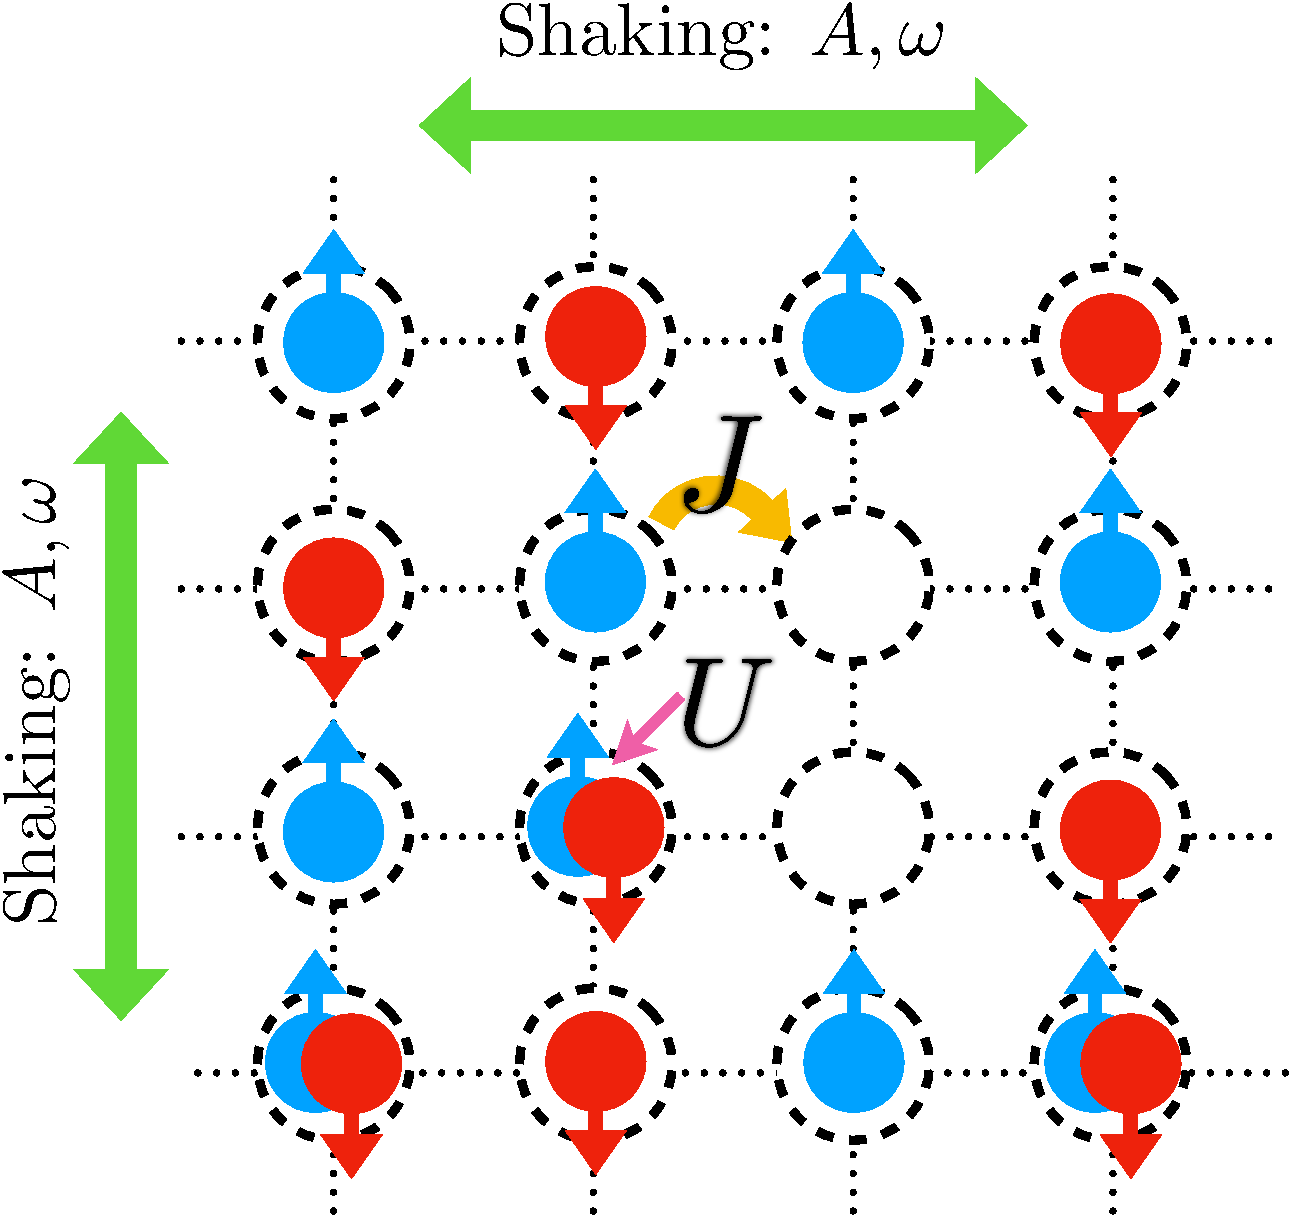
\includegraphics[width=1.0\columnwidth]{diffusion/schematic}
\caption{CDW 和 SDW 态的示意图。上栏为自旋密度波 SDW 的例子。下栏为电荷密度波 CDW 的例子。(取自\inlinecite{diffusion})}
\label{fig:diffusion:schematic}
\end{figure}

将上述三个引理结合起来,并利用我们在 \ref{sec:dynsymm} 节证明的受对称性保护的动力学对称性(定理 \ref{thm:dynsymm}),我们可以证明在半填充的二分 Fermi Hubbard 模型中,局域电荷密度和局域自旋密度之间存在严格映射,其期望值存在精确关系。

\begin{theorem}\label{thm:diffusion}
在半填充的二分 Fermi Hubbard 模型中,局域电荷密度在电荷密度波态的演化下的期望值,与局域自旋密度在自旋密度波的演化下的期望值,之间存在严格的精确关系。即,
\begin{align}
\langle \hat{n}_i(t)\rangle_{\psi_1} = 1 - \langle \hat{S}_i(t)\rangle_{\psi_2}.
\end{align}
其中 $|\psi_1\rangle$ 和 $|\psi_2\rangle$ 分别出自 CDW 类 和 SDW 类。
\end{theorem}

\begin{figure}[!htb]
\centering
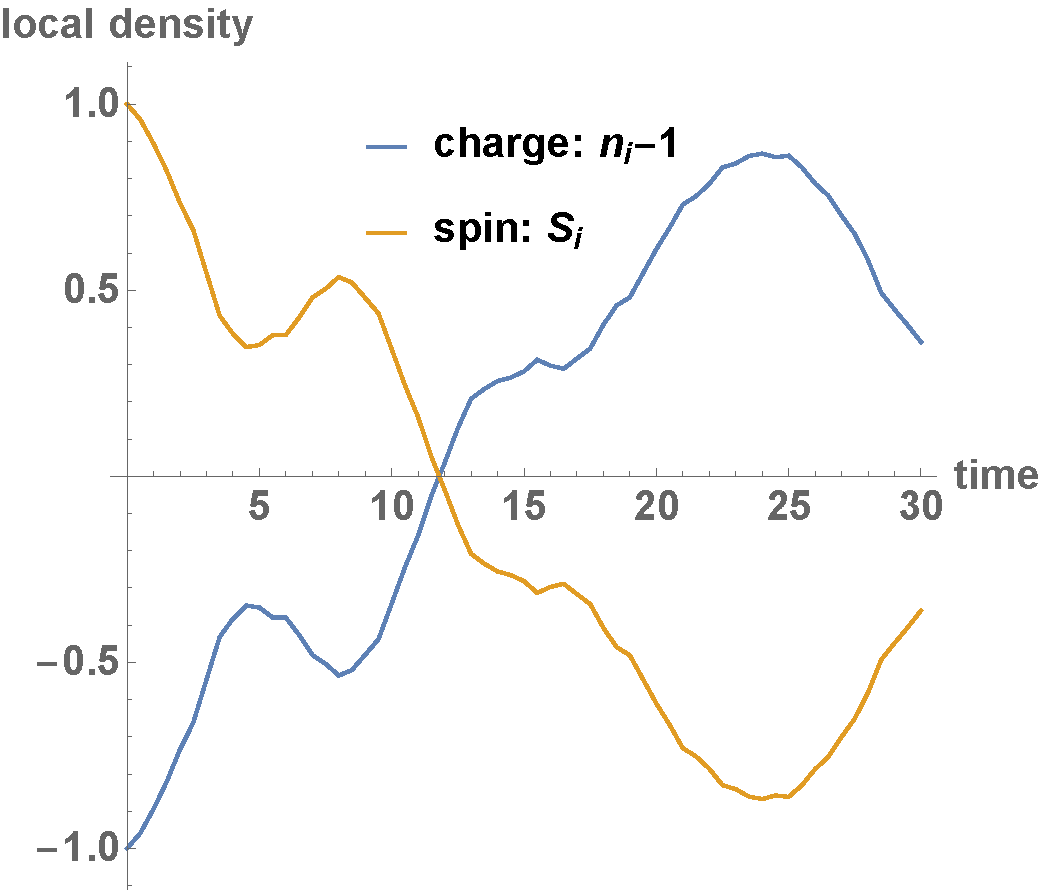
\includegraphics[width=0.7\columnwidth]{chap3_dynm/fhed}
\caption{Fermi Hubbard 严格对角化验证局域电荷密度与局域电荷密度的动力学演化。严格对角化在4个格点上进行,模型参数 $U/J=10$。取 $i=3$ 的格点进行测量。}
\label{fig:diffusion:fhed}
\end{figure}

\begin{proof}
对于二分的晶格,存在幺正变换 $\hat{W}$,
\begin{align}
W\hat{c}_{i\sigma}W^{-1} = (-1)^i\hat{c}_{i\sigma}
\end{align}
和时间反演变换 $\hat{R}$,使得 $S=RW$ 满足定理 \ref{thm:dynsymm} 中的条件,即
\begin{align}
\{S, \hat{H}_0\} = 0\\
[S, \hat{H}_I]=0
\end{align}
并且,局域电荷密度算符和局域自旋密度算符均具有 $S$-对称性,上面定义的 CDW 态 和 SDW 态均是 $S$-不变的。因此,利用上面三个引理,可得
\begin{align}
\langle \hat{n}_i(t)\rangle_{\psi_1, +U} 
&= \langle \psi_1|e^{iH(+U)t}\hat{n}_ie^{-iH(+U)t}|\psi_1\rangle \notag\\
&= \langle \psi_1|e^{iH(+U)t}\mathcal{P}^{-1}\mathcal{P}\hat{n}_i\mathcal{P}^{-1}\mathcal{P}e^{-iH(+U)t}|\psi_1\rangle \notag\\
&= \langle \psi_2|e^{iH(-U)t} (1-\hat{S}_i) e^{-iH(-U)t}|\psi_2\rangle \\
&= 1 - \langle \psi_2|e^{iH(-U)t} \hat{S}_i e^{-iH(-U)t}|\psi_2\rangle \notag\\
&= 1 - \langle \hat{S}_i(t) \rangle_{\psi_2, -U}, \notag 
\end{align}
再利用定理 \ref{thm:dynsymm},可得
\begin{align}
\langle \hat{S}_i(t)\rangle_{\psi_2, -U} = \langle \hat{S}_i(t)\rangle_{\psi_2, +U},  
\end{align}
因此有
\begin{align}\label{eq:n=1-S}
\langle \hat{n}_i(t)\rangle_{\psi_1, +U} = 1 - \langle \hat{S}_i(t)\rangle_{\psi_2, +U}. 
\end{align}
证毕。
\end{proof}

对于定理 \ref{thm:diffusion},我们进行了严格对角化的数值验证,见图 \ref{fig:diffusion:fhed}。



\subsection{偏离半满和更一般的观测量的推广}
上面为了叙述与证明的简便,假设了体系处于半满,并且只考虑了局域电荷密度观测量和局域自旋密度观测量的动力学演化行为。事实上,上述定理的半填充的约束完全可以放开,对观测量的定义也可以更广泛。。在文章\inlinecite{diffusion} 中,我们对定理做了更一般的表述。而证明的步骤仍是利用粒子空穴变换+受对称性保护的动力学对称性两步。参考图 \ref{fig:diffusion:results} 的证明示意图。
\begin{figure}[!htb]
\centering
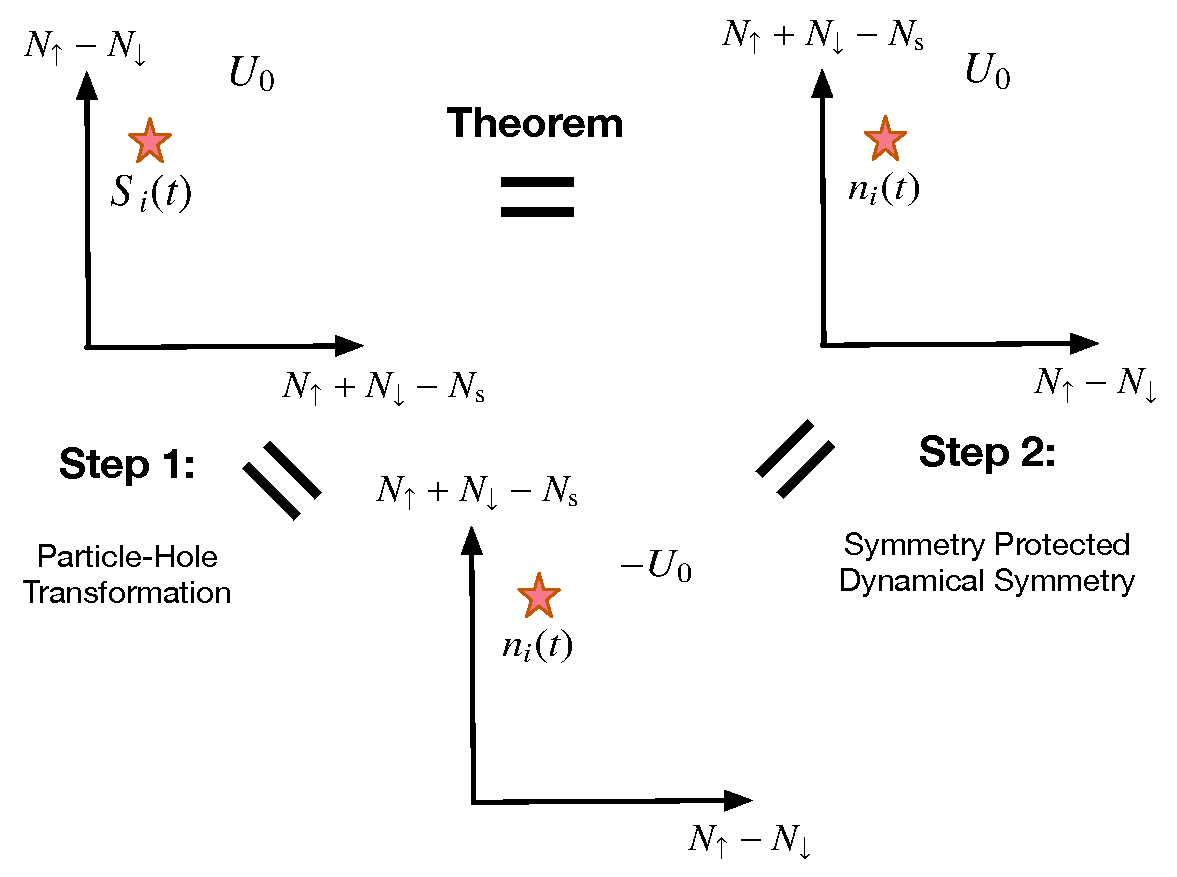
\includegraphics[width=1.0\columnwidth]{diffusion/results}
\caption{定理 \ref{thm:diffusion} 的证明示意图。 定理的证明分为两步:第一步是利用粒子空穴变换将$+U$的模型映射到$-U$的模型,同时将局域自旋密度量和局域电荷密度量进行映射;第二步是利用定理 \ref{thm:dynsymm} 中的受对称性保护的动力学对称性,将 $-U$ 的模型映射回 $+U$ 的模型,而同时特定可观测算符在特定初态下的动力学演化过程也被映射过来。(取自\inlinecite{diffusion})}
\label{fig:diffusion:results}
\end{figure}

对于更一般的情况,可观测量不再局限于局域电荷密度算符和局域自旋密度算符,凡是满足定理 \ref{thm:dynsymm} 所述,具有 $S$-对称性的算符均有类似的精确关系存在。对于态的定义也不局限于半填充,甚至不局限于定义\ref{def:state12}中的两类 CDW 和 SDW。凡是具有能相互映射的 $S_i$ 与 $1-n_i$ 的期望值的两个态均可以。


\subsection{温度效应}
还有一种推广是考虑温度的效应。当系统处于有限温时,体系不再是纯态。上面对态的讨论需改为对密度矩阵 $\rho=e^{-\beta H}$ 的讨论,这里 $\beta=1/T$,$T$ 是系统的温度。这种情况下可观测量的期望值为 
\begin{align}
n = tr(\rho\hat{n})
\end{align}
如果我们要证明局域电荷密度的动力学过程与居于自旋密度的动力学过程之间存在对称性,那我们就需要从上述密度算符 $\rho$ 和期望值 $n$ 出发进行证明,这不是一件容易的事情(而且很可能并不存在严格的对称性了)。然而,有一种特殊的情况我们可以证明,那就是无穷高温的情况。一方面
\begin{align}
\mathcal{P}e^{-\beta H(+U)}\mathcal{P}^{-1} = e^{-\beta H(-U)}
\end{align}
另一方面,
\begin{align}
Se^{-\beta H(-U)}S^{-1} = e^{\beta H(+U)}
\end{align}
两者的联合变换使得
\begin{align}
\mathcal{P}S: e^{-\beta H} \leftrightarrow e^{\beta H}
\end{align}
无穷高温时,$\beta=0$,因此有
\begin{align}
e^{-\beta H} = e^{\beta H}
\end{align}
因此,在 $\mathcal{P}$ 和 $S$ 的联合变换下,无穷高温的混态系综 $\rho$ 被影射为它自己。而定理其他部分证明不变,因此这种情况下定理依然成立,局域电荷密度的动力学过程和局域自旋密度的动力学过程之间仍然可以相互映射。



\subsection{输运方程的对称性}
考虑局域密度观测量的扩散过程。
\begin{align}
    \partial_tn + \nabla\cdot\vec{j} = 0, \\
    \vec{j} = -D_c\nabla n. 
\end{align}
这里 $\vec{j}$ 是局域的流。从上式可推出扩散方程,
\begin{align}
    \partial_tn-D_c\nabla^2n = 0 
\end{align}
对于特定满足条件的初态,根据 (\ref{eq:n=1-S}) 式,则有
\begin{align}
    \partial_t\langle\hat{n}_i(t)\rangle_{\psi_1, +U} &= -\partial_t\langle\hat{S}_i(t)\rangle_{\psi_2, +U} \\ 
    \nabla^2\langle\hat{n}_i(t)\rangle_{\psi_1, +U} &= -\nabla^2\langle\hat{S}_i(t)\rangle_{\psi_2, +U}
\end{align}






\subsection{一类 Fermi-Hubbard 模型中的 SO(4) 对称性与电子-空穴对称性}\label{sec:so4}

在这里我们来讨论一类 Fermi Hubbard 模型所具有的 SO(4) 对称性\cite{yang1990}与电子空穴对称性。Fermi Hubbard 模型具有 SO(4) 对称性最早由杨振宁先生和张首晟教授在 \inlinecite{yang1990} 文章中予以证明,现已成为 Hubbard 模型研究领域的常识性的知识。事实上,通过 \ref{sec:diffusion} 上面提到的粒子空穴变换,即 
\begin{align}
    \mathcal{P} : \  \  
    & \hat{c}_{i\uparrow} \rightarrow (-1)^{i} \hat{c}_{i\uparrow}^{\dagger},  \nonumber\\
    & \hat{c}_{i\downarrow} \rightarrow \hat{c}_{i\downarrow}. 
\end{align}
以及上面证明过的引理 \ref{lemma1}(即对半填充的模型,在该变换下 $+U$ 的模型被映射为 $-U$ 的模型,反之亦然),很容易证明对于半填充的情况,该模型具有 $SO(4)$ 对称性。
首先,Fermi Hubbard 模型具有自旋-SU(2) 对称性,而上述映射将该 SU(2) 映射为 电荷-SU(2),因此同一个模型具有 SU(2)$\times$SU(2)=SO(4) 的对称性。

% 不过,半填充的约束在此处仍非必要。体系半填充就像体系是自旋平衡的一样,都是对于态的约束,这样的约束在讨论模型(哈密顿量)的对称性时完全可以放开。就像本节开头提到的,半填充只是调节化学势 $\mu$ 到 $\mu=N/2$ 的另一种表述,这样的常数项本身并不影响模型的对称性。作为更一般的情况,我们这里将该 SO(4) 对称性进行更普适地形式化表述。

% Fermi Hubbard 模型哈密顿量写作
% \begin{align}
%     \hat{H} = \sum_{\langle i,j\rangle,\sigma} -t\hat{c}_{i\sigma}^{\dagger}\hat{c}_{j\sigma} + \sum_{i} U \hat{n}_{i\uparrow}\hat{n}_{i\downarrow} 
% \end{align}

更严格的,对于半填充 Fermi Hubbard 模型,
\begin{align}
    \hat{H} = \sum_{\langle i,j\rangle,\sigma} -t\hat{c}_{i\sigma}^{\dagger}\hat{c}_{j\sigma} + \sum_{i} U \left(\hat{n}_{i\uparrow}-\dfrac{1}{2}\right)\left(\hat{n}_{i\downarrow}-\frac{1}{2}\right) 
\end{align}
可验证其具有如下定义的自旋SU(2)对称性和电荷SU(2)对称性。

\begin{definition}\label{def:spinsu2}
自旋$su(2)$生成元定义如下
\begin{align}\label{eq:spinsu2}
    \hat{S}_z &= \frac{1}{2}\sum_{i}\hat{c}_{i\uparrow}^{\dagger}\hat{c}_{i\uparrow}-\hat{c}_{i\downarrow}\hat{c}_{i\downarrow}, \\  
    \hat{S}_{+} &= \sum_{i}\hat{c}_{i\uparrow}^{\dagger}\hat{c}_{i\downarrow}, 
\end{align}
\begin{align}
    \hat{S}_{-} = \hat{S}_{+}^{\dagger}, \  \  
    \hat{S}_{x} = \frac{\hat{S}_{+}+\hat{S}_{-}}{2}, \  \  
    \hat{S}_{y} = \frac{\hat{S}_{+}-\hat{S}_{-}}{2i},
\end{align}
\end{definition}
容易验证,
\begin{align}
[\hat{H}, \hat{S}_{\alpha}]=0, \quad \alpha=x,y,z
\end{align}

\begin{definition}\label{def:spinsu2}
电荷$su(2)$生成元定义如下
\begin{align}
    \hat{L}_z &= -\frac{1}{2}\sum_{i}\hat{c}_{i\uparrow}^{\dagger}\hat{c}_{i\uparrow}+\hat{c}_{i\downarrow}^{\dagger}\hat{c}_{i\downarrow}+\frac{1}{2}N, \\ 
    \hat{L}_{+} &= \sum_{i}(-1)^i\hat{c}_{i\uparrow}\hat{c}_{i\downarrow} = \sum_{i}\exp(i\mathbf{Q}\cdot\mathbf{x}_i)\hat{c}_{i\uparrow}\hat{c}_{i\downarrow}
\end{align}
这里 $\mathbf{Q} = (\pi, \pi)$, $N$ 是总格点数,
\begin{align}
    \hat{L}_{-} = \hat{L}_{+}^{\dagger}, \  \  
    \hat{L}_{x} = \frac{\hat{L}_{+}+\hat{L}_{-}}{2}, \  \  
    \hat{L}_{y} = \frac{\hat{L}_{-}-\hat{L}_{-}}{2i}. 
\end{align}
\end{definition}
容易验证,
\begin{align}
[\hat{H}, \hat{L}_{\alpha}]=0, \quad \alpha=x,y,z
\end{align}


另外,半填充的 Fermi Hubbard 模型还具有粒子空穴对称性。定义如下粒子空穴变换
\begin{align}
\hat{C}: \hat{c}_{i\sigma} \rightarrow (-1)^i\hat{c}_{i\sigma}^{\dagger}
\end{align}
容易验证,$[\hat{H}, \hat{C}]=0$。



除了通常的 Fermi Hubbard 模型,还有一些推广的 Fermi Hubbard 模型也具有上述两个对称性。这里,作为一个例子,我们来讨论如下的有效模型,该模型将在第 \ref{sec:floqhubb} 节中被更细致地讨论。
\begin{align}
\hat{H}_{\text{eff}} &= - \sum_{\langle i,j\rangle, \sigma} 
\left(J_0[(1-\hat{n}_{i\bar\sigma})(1-\hat{n}_{j\bar\sigma}) + \hat{n}_{i\bar\sigma}\hat{n}_{j\bar\sigma}]
+J_1[(-1)^l(1-\hat{n}_{i\bar\sigma})\hat{n}_{j\bar\sigma} + \hat{n}_{i\bar\sigma}(1-\hat{n}_{j\bar\sigma})]\right)
\hat{c}_{i\sigma}^{\dagger}\hat{c}_{j\sigma} \nonumber\\
& \quad + \tilde{U}\sum_{i}\left(\hat{n}_{i\uparrow}-\frac{1}{2}\right)\left(\hat{n}_{i\downarrow}-\frac{1}{2}\right)
\end{align}
% 对于 $J_0\neq J_1$ 的情况,
可以直接验证:

\begin{itemize}

\item $l$ 为偶数时,
\begin{align}
[\hat{H}_{\text{eff}}, \hat{S}_{\alpha}] &= 0, \quad \alpha=x,y,z \\
[\hat{H}_{\text{eff}}, \hat{L}_{\alpha}] &= 0, \quad \alpha=x,y,z 
\end{align}
因此模型具有 SO(4) 对称性。
\begin{align}
[\hat{H}_{\text{eff}}, \hat{C}]=0
\end{align}
因此模型具有粒子空穴对称性。

\item $l$ 为奇数时,
\begin{align}
[\hat{H}_{\text{eff}}, \hat{S}_{\alpha}] &= 0, \quad \alpha=x,y,z
[\hat{H}_{\text{eff}}, \hat{L}_{\alpha}] &= 0, \quad \alpha=x,y,z 
\end{align}
但
\begin{align}
[\hat{H}_{\text{eff}}, \hat{L}_{\alpha}] &= 0, \quad \alpha=x,y,z 
\end{align}
不再成立。
因此模型具有 自旋-SU(2) 对称性,但不具有 电荷-SU(2) 对称性。因此也不具有 SO(4) 对称性。

引入二分晶格变换 $\hat{S}$ (参考上一节内容),有
\begin{align}
[\hat{H}_{\text{eff}}, \hat{C}\hat{S}]=0
\end{align}
因此模型具有粒子空穴对称性。

\end{itemize}



